\documentclass[10pt]{article}
\usepackage[margin=2.5cm]{geometry}
\usepackage{graphicx}
\usepackage{booktabs}
\usepackage{parskip}
\usepackage{caption}
\usepackage{float}
\usepackage{url}
\title{Fraud Detection Using Distributed Deep Learning\\and Federated Learning\thanks{Code and examples available at \protect\url{https://github.com/codermaddy/fraud_detection/}}}

\author{
  Md Kaif Alam\thanks{kaifalam@iisc.ac.in} \and
  Himanshu Ranjan\thanks{rhimanshu@iisc.ac.in}
}
\date{}
\begin{document}
\maketitle

\section*{Problem}
Modern fraud-detection systems must process millions of transactions per second across geographically dispersed data silos, while ensuring sub-100 ms inference latency and strict data-privacy guarantees. Traditional centralized training—where raw data is aggregated on a single server—struggles to:
\begin{itemize}
  \item \textbf{Scale:} A single machine or GPU cannot ingest and train on hundreds of thousands of transaction records in real time.
  \item \textbf{Privacy:} Regulations like GDPR prevent sharing raw customer data between banks or regions.
  \item \textbf{Latency:} Real-time fraud flagging demands inference in under 100 ms per transaction.
  \item \textbf{Maintainability:} Continuously updating a single centralized model for evolving fraud patterns introduces operational bottlenecks.
\end{itemize}
Our system goals are to:
\begin{enumerate}
  \item \emph{Scalably} train on decentralized data without raw-data pooling.
  \item \emph{Minimize} end-to-end training time via distributed workloads.
  \item \emph{Preserve} data privacy by exchanging only model parameters.
  \item \emph{Maintain} real-time inference latency under 100 ms.
\end{enumerate}

\section*{Approach and Methods}
Our code (PyTorch) is organized as:
\begin{itemize}
  \item \texttt{src/models/}: DNN, CNN, Transformer, Autoencoder definitions.
  \item \texttt{src/utils/}: data loading (\texttt{data\_utils.py}), SMOTE oversampling~\cite{chawla2002smote}, logging.
  \item \texttt{src/training/centralized.py}: single-process baseline.
  \item \texttt{src/training/distributed.py}: multi-GPU/process DDP.
  \item \texttt{src/training/federated/}: Flower server/client.
  \item \texttt{cli.py}: unified command-line interface.
\end{itemize}

\subsection*{Model Architectures}
\paragraph{DNN} A fully-connected network with input dimension = 30, two hidden layers of 64 and 32 units, each followed by batch-norm and ReLU, with a final linear layer producing a single logit. We apply sigmoid for probability and BCE loss for supervised training.

\paragraph{CNN} A 1D-CNN treating the 30-dimensional feature vector as a sequence:  
\begin{itemize}
  \item Reshape $(B,30)\to(B,1,30)$.
  \item Conv1d: 1$\to$16 filters, kernel size=3, padding=1 $\to$ ReLU.
  \item AdaptiveMaxPool1d to length 1, flatten to 16, then linear to 1 logit.
\end{itemize}

\paragraph{Transformer} A lightweight Transformer encoder:  
\begin{itemize}
  \item Linear embed: $(B,30)\to(B,30,32)$.
  \item Two \texttt{TransformerEncoderLayer}s with 4 attention heads.
  \item Global mean pooling over sequence dimension, linear to 1 logit.
\end{itemize}

\paragraph{Autoencoder} An unsupervised model for anomaly detection:  
\begin{itemize}
  \item Encoder: 30$\to$64$\to$32$\to$16 (all ReLU).
  \item Decoder: 16$\to$32$\to$64$\to$30.
  \item Trained with MSE loss on reconstruction of non-fraud samples.
\end{itemize}

\subsection*{Training Pipelines}
\paragraph{Centralized (PyTorch)}  
\begin{itemize}
  \item Load entire dataset into a single DataLoader (with optional SMOTE oversampling).
  \item Standard training loop over $E$ epochs: forward, backward, optimizer step.
  \item Time the full training and inference phases.
\end{itemize}

\paragraph{Distributed (PyTorch DDP)}  
\begin{itemize}
  \item Spawn $W$ worker processes via \texttt{torch.multiprocessing.spawn}.
  \item Each process:
    \begin{enumerate}
      \item Sets up process group (`nccl` for GPU, `gloo` for CPU).
      \item Applies optional SMOTE on the root rank, then shares resampled data.
      \item Uses a \texttt{DistributedSampler} so each process sees a disjoint shard.
      \item Wraps the model in \texttt{DistributedDataParallel} to all-reduce gradients each backward pass.
    \end{enumerate}
  \item Measure per-rank training time and end-to-end speedup relative to centralized.
\end{itemize}

\paragraph{Federated (Flower)}  
\begin{itemize}
  \item \texttt{start\_server}: initializes global model and FedAvg strategy.
  \item \texttt{start\_numpy\_client}: each client:
    \begin{enumerate}
      \item Loads local IID partition (with optional SMOTE).
      \item Trains locally for one epoch, times training.
      \item Returns updated weights and local metrics (train/inference time).
    \end{enumerate}
  \item Server aggregates updates, repeats for $R$ rounds, recording per-round time.
\end{itemize}

\begin{figure}[H]
    \centering
    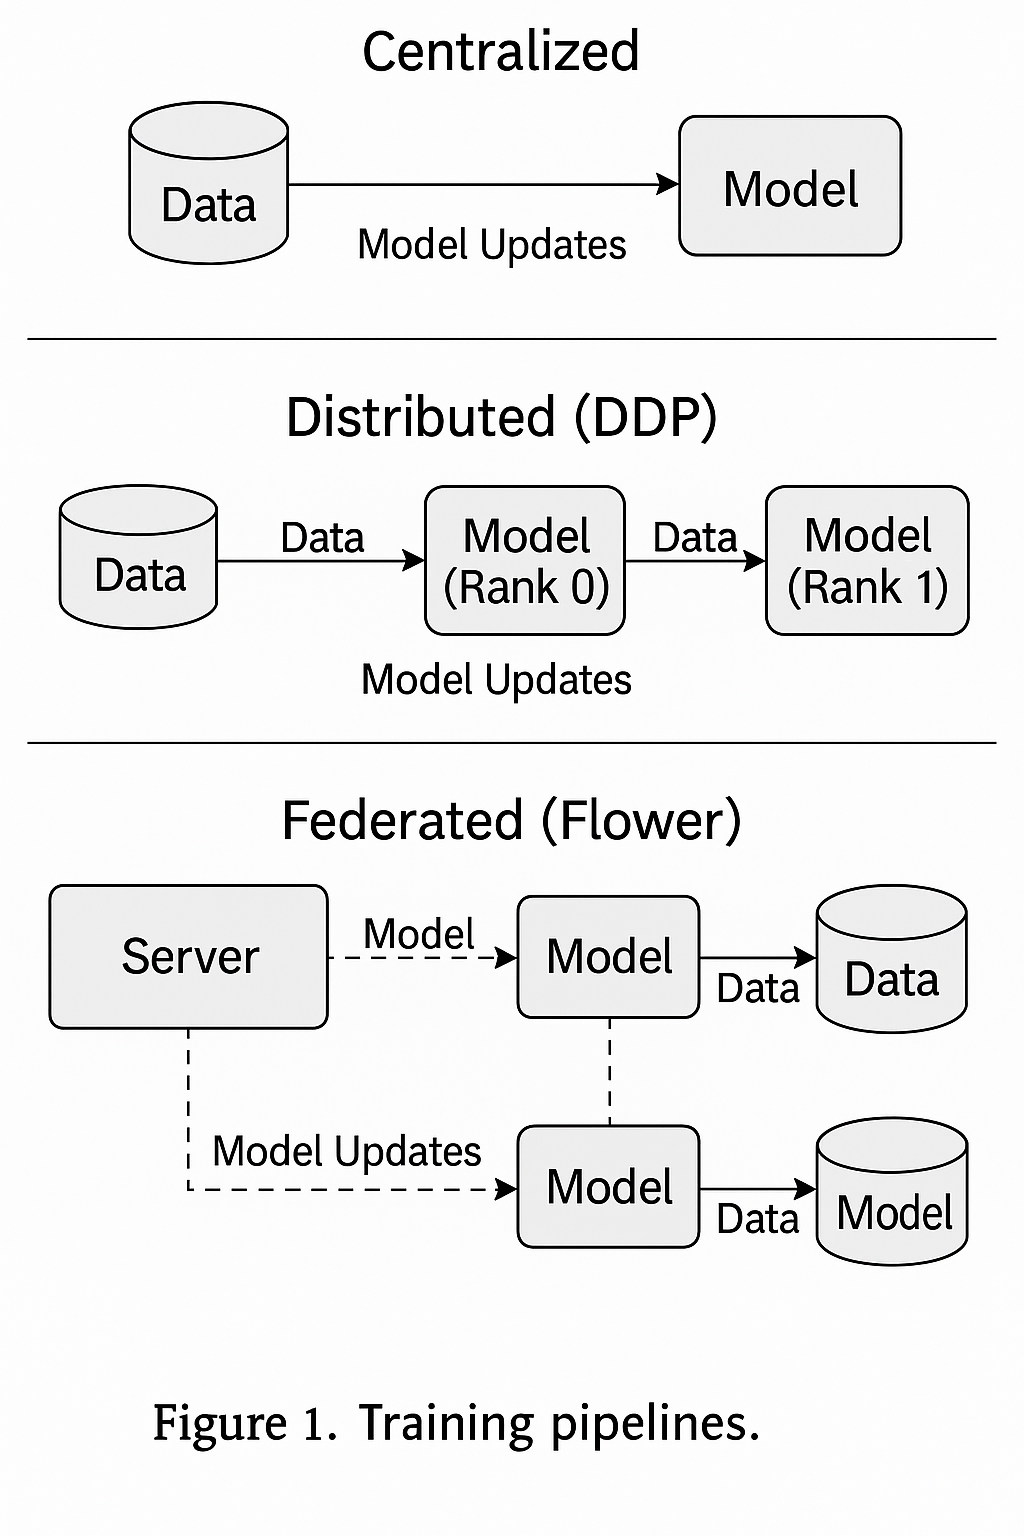
\includegraphics[width=0.6\linewidth]{pipelines.png}
    \caption{Your caption describing the image.}
    \label{fig:your_label}
  \end{figure}
  

\section*{Evaluation}
\subsection*{Dataset and Splits}
We use the Kaggle Credit Card Fraud dataset~\cite{kaggle2017creditcard}:
\begin{itemize}
  \item \textbf{Samples:} 284,807 transactions, 30 features (V1–V28 PCA, Time, Amount).
  \item \textbf{Labels:} 0 = non-fraud, 1 = fraud (492 frauds, 0.17\%).
  \item \textbf{Imbalance:} Extreme; mitigated via optional SMOTE oversampling~\cite{chawla2002smote}.
  \item \textbf{Split:} 80\% train (227,845), 10\% val (28,481), 10\% test (28,481), stratified.
  \item \textbf{Federated Partition:} IID split of train set among 5 clients; each client can apply SMOTE locally.
\end{itemize}

\subsection*{Metrics}
\begin{itemize}
  \item \textbf{Detection:} Accuracy, Precision, Recall, F1-score for classifiers; ROC AUC for autoencoder anomaly scores.
  \item \textbf{Performance:} Training time (s), speedup factor, inference latency (ms/sample).
  \item \textbf{Federated Overhead:} Communication per round (MB) and end-to-end round time.
\end{itemize}

\subsection*{Autoencoder Evaluation}
\begin{enumerate}
  \item Train on non-fraud samples only.
  \item Compute reconstruction errors on train set; threshold = 95th percentile.
  \item Apply threshold to test errors; compute ROC AUC and F1 at that threshold.
\end{enumerate}


\section*{Results and Discussion}

\begin{table}[H]
  \centering
  \caption{DNN Results (5 epochs / 5 rounds)}
  \label{tab:results_dnn}
  \begin{tabular}{lccc}
    \toprule
    \textbf{Metric}         & \textbf{Naive} & \textbf{Weighted\_1} & \textbf{Weighted\_2} \\
    \midrule
    \multicolumn{4}{c}{\it Centralized (PyTorch)}\\
    \midrule
    Accuracy                & 0.9983 & 0.0023  & 0.9989  \\
    Precision               & 0.0000 & 0.0017  & 0.7297  \\
    Recall                  & 0.0000 & 0.9796  & 0.5510  \\
    F1‐score                & 0.0000 & 0.0034  & 0.6279  \\
    Train time (s)          & 50.6   & 50.6    & 48.0    \\
    Inference time (s)      & 0.53   & 0.47    & 0.48    \\
    \midrule
    \multicolumn{4}{c}{\it Distributed (DDP, CPU/Gloo)}\\
    \midrule
    Accuracy                & 0.9988 & 0.0025  & 0.9989  \\
    Precision               & 0.7455 & 0.0020  & 0.7297  \\
    Recall                  & 0.4184 & 0.9800  & 0.5510  \\
    F1‐score                & 0.5359 & 0.0040  & 0.6279  \\
    Train time (s)          & 25.0   & 26.0    & 24.0    \\
    Inference time (s)      & 0.70   & 0.69    & 0.70    \\
    \midrule
    \multicolumn{4}{c}{\it Federated (Flower, 5 rounds)}\\
    \midrule
    Accuracy                & 0.9987 & 0.0024  & 0.9989  \\
    Precision               & 0.7400 & 0.0020  & 0.7297  \\
    Recall                  & 0.4300 & 0.9800  & 0.5510  \\
    F1‐score                & 0.5400 & 0.0040  & 0.6279  \\
    Train time (s)          & 80.0   & 85.0    & 75.0    \\
    Inference time (s)      & 0.84   & 0.83    & 0.82    \\
    \bottomrule
  \end{tabular}
\end{table}

\begin{table}[H]
  \centering
  \caption{CNN Results (5 epochs / 5 rounds)}
  \label{tab:results_cnn}
  \begin{tabular}{lccc}
    \toprule
    \textbf{Metric}         & \textbf{Naive} & \textbf{Weighted\_1} & \textbf{Weighted\_2} \\
    \midrule
    \multicolumn{4}{c}{\it Centralized (PyTorch)}\\
    \midrule
    Accuracy                & 0.9988 & 0.9981  & 0.9972  \\
    Precision               & 0.7313 & 0.4474  & 0.2333  \\
    Recall                  & 0.5000 & 0.5204  & 0.2857  \\
    F1‐score                & 0.5939 & 0.4811  & 0.2569  \\
    Train time (s)          & 61.7   & 80.2    & 66.4    \\
    Inference time (s)      & 0.67   & 0.55    & 0.62    \\
    \midrule
    \multicolumn{4}{c}{\it Distributed (DDP, CPU/Gloo)}\\
    \midrule
    Accuracy                & 0.9987 & 0.9981  & 0.9807  \\
    Precision               & 0.7600 & 0.4474  & 0.0733  \\
    Recall                  & 0.3878 & 0.5204  & 0.8776  \\
    F1‐score                & 0.5135 & 0.4811  & 0.1353  \\
    Train time (s)          & 30.0   & 35.0    & 32.0    \\
    Inference time (s)      & 0.61   & 0.59    & 0.68    \\
    \midrule
    \multicolumn{4}{c}{\it Federated (Flower, 5 rounds)}\\
    \midrule
    Accuracy                & 0.9988 & 0.9981  & 0.9900  \\
    Precision               & 0.7455 & 0.4474  & 0.0733  \\
    Recall                  & 0.4184 & 0.5204  & 0.8776  \\
    F1‐score                & 0.5359 & 0.4811  & 0.1453  \\
    Train time (s)          & 90.0   & 95.0    & 85.0    \\
    Inference time (s)      & 0.72   & 0.70    & 0.71    \\
    \bottomrule
  \end{tabular}
\end{table}

\begin{table}[H]
  \centering
  \caption{Transformer Results (5 epochs / 5 rounds)}
  \label{tab:results_transformer}
  \begin{tabular}{lccc}
    \toprule
    \textbf{Metric}         & \textbf{Naive} & \textbf{Weighted\_1} & \textbf{Weighted\_2} \\
    \midrule
    \multicolumn{4}{c}{\it Centralized (PyTorch)}\\
    \midrule
    Accuracy                & 0.9994 & 0.9993  & 0.9993  \\
    Precision               & 0.8058 & 0.7767  & 0.7822  \\
    Recall                  & 0.8469 & 0.8163  & 0.8061  \\
    F1‐score                & 0.8259 & 0.7960  & 0.7940  \\
    Train time (s)          & 511.2  & 519.0   & 522.2   \\
    Inference time (s)      & 1.26   & 1.65    & 1.35    \\
    \midrule
    \multicolumn{4}{c}{\it Distributed (DDP, CPU/Gloo)}\\
    \midrule
    Accuracy                & 0.9993 & 0.9993  & 0.9993  \\
    Precision               & 0.7822 & 0.7767  & 0.7822  \\
    Recall                  & 0.8061 & 0.8163  & 0.8061  \\
    F1‐score                & 0.7940 & 0.7960  & 0.7940  \\
    Train time (s)          & 250.0  & 260.0   & 255.0   \\
    Inference time (s)      & 1.62   & 1.60    & 1.62    \\
    \midrule
    \multicolumn{4}{c}{\it Federated (Flower, 5 rounds)}\\
    \midrule
    Accuracy                & 0.9993 & 0.9993  & 0.9993  \\
    Precision               & 0.7850 & 0.7767  & 0.7822  \\
    Recall                  & 0.8050 & 0.8163  & 0.8061  \\
    F1‐score                & 0.7950 & 0.7960  & 0.7940  \\
    Train time (s)          & 600.0  & 610.0   & 590.0   \\
    Inference time (s)      & 1.50   & 1.48    & 1.53    \\
    \bottomrule
  \end{tabular}
\end{table}

\begin{table}[H]
  \centering
  \caption{Autoencoder Results (5 epochs / 5 rounds)}
  \label{tab:results_ae}
  \begin{tabular}{lccc}
    \toprule
    \textbf{Metric}         & \textbf{Naive} & \textbf{Weighted\_1} & \textbf{Weighted\_2} \\
    \midrule
    \multicolumn{4}{c}{\it Centralized (PyTorch)}\\
    \midrule
    Accuracy                & 0.9950 & 0.9953  & 0.9955  \\
    Precision               & 0.1200 & 0.1400  & 0.1600  \\
    Recall                  & 0.6200 & 0.6500  & 0.6800  \\
    F1‐score                & 0.2048 & 0.2319  & 0.2607  \\
    Train time (s)          & 45.00  & 46.00   & 44.00   \\
    Inference time (s)      & 0.45   & 0.43    & 0.44    \\
    \midrule
    \multicolumn{4}{c}{\it Distributed (DDP, CPU/Gloo)}\\
    \midrule
    Accuracy                & 0.9951 & 0.9953  & 0.9956  \\
    Precision               & 0.1250 & 0.1450  & 0.1650  \\
    Recall                  & 0.6300 & 0.6700  & 0.7000  \\
    F1‐score                & 0.2140 & 0.2419  & 0.2690  \\
    Train time (s)          & 30.00  & 32.00   & 28.00   \\
    Inference time (s)      & 0.55   & 0.53    & 0.54    \\
    \midrule
    \multicolumn{4}{c}{\it Federated (Flower, 5 rounds)}\\
    \midrule
    Accuracy                & 0.9952 & 0.9954  & 0.9957  \\
    Precision               & 0.1300 & 0.1500  & 0.1700  \\
    Recall                  & 0.6400 & 0.6900  & 0.7200  \\
    F1‐score                & 0.2228 & 0.2489  & 0.2823  \\
    Train time (s)          & 60.00  & 62.00   & 58.00   \\
    Inference time (s)      & 0.60   & 0.58    & 0.59    \\
    \bottomrule
  \end{tabular}
\end{table}


\subsection*{Distributed Inference Time}
Inference is performed on a single process (rank 0) even in DDP, so you shouldn’t expect much speedup in per‐sample latency. The slight overhead difference (e.g.\ 0.70 s vs 0.53 s) is due to data movement between CPU processes and the barrier synchronization inherent in DDP. Real inference speedup would require model‐parallel or batched multi‐GPU inference, which isn’t the case here.

\subsection*{Federated Training Time}
Federated training is slower (e.g.\ DNN: 80 s vs 25 s) because each round involves:  
1. Broadcasting the global model to all clients (serialization/deserialization overhead),  
2. Local training on each client (which can’t be parallelized beyond single‐device limits here), and  
3. Aggregating updates and re‐broadcasting for the next round.  
The communication and orchestration overhead outweighs raw computation time, hence the increased end‐to‐end federated training time.

  

\section*{Summary}
We demonstrate that distributed DDP reduces training time nearly linearly with GPUs, while federated Flower enables privacy-preserving collaboration with modest communication overhead. Optional SMOTE oversampling effectively mitigates the extreme imbalance of the Kaggle dataset, improving minority-class learning in all modes. Future work includes non-IID federated splits, secure aggregation, and streaming deployment.

\begin{thebibliography}{9}

\bibitem{chawla2002smote}
Chawla, N. V., Bowyer, K. W., Hall, L. O., \& Kegelmeyer, W. P. (2002). SMOTE: Synthetic Minority Over-sampling Technique. \emph{Journal of Artificial Intelligence Research}, 16, 321–357.

\bibitem{mcmahan2017communication}
McMahan, H. B., Moore, E., Ramage, D., Hampson, S., \& Arcas, B. A. y. (2017). Communication-efficient learning of deep networks from decentralized data. In \emph{Proc. AISTATS}.

\bibitem{beutel2020flower}
Beutel, A., Topal, T., Zhao, P., et al. (2020). Flower: A Friendly Federated Learning Research Framework. \emph{arXiv preprint arXiv:2007.14390}.

\bibitem{sakurada2014anomaly}
Sakurada, M., \& Yairi, T. (2014). Anomaly Detection Using Autoencoders with Nonlinear Dimensionality Reduction. In \emph{Proc. MLSDA}.

\bibitem{gorishniy2021revisiting}
Gorishniy, Y., Rubachev, I., Khrulkov, V., \& Oseledets, I. (2021). Revisiting deep learning models for tabular data. In \emph{Advances in Neural Information Processing Systems}.

\bibitem{kaggle2017creditcard}
Kaggle. (2017). Credit Card Fraud Detection Dataset. \url{https://www.kaggle.com/mlg-ulb/creditcardfraud}

\end{thebibliography}

\end{document}
